% !TeX spellcheck = en
\chapter{Python Projects} \label{sec:Python}

    \FloatBarrier
    \section{Installing Python Interpreter}

Visual Studio supports Python projects and solutions by selecting during the Visual Studio installation the \textbf{Python Development} workload. If we do not have installed it yet, we can always do it when needed thanks to the Visual Studio Installer tool. In order to do that:

\begin{enumerate}
	\item Open \textit{Visual Studio Installer} application as an administrator.
	%\item It may happen that the program requires an upgrade. Click on \textit{Update} and wait for the installation to finish.
	\item Click on \textit{Modify} on the space reserved for your currently version of Visual Studio (Figure \ref{fig:vsi:list}). %If the \textit{Update} button were to appear instead, click on \textit{Update} and wait for the installation to complete, the \textit{Modify} button should be now available.
	\item Now, in the \textit{Workloads} tab, select \textit{Python Development}. Check that the first three elements of the optional modules to be installed are selected (\texttt{Python 3 xx-bit (3.x.x)} included), it can be checked on the right part of the window as it is shown in the Figure \ref{fig:vsi:mods}.
	\item Click on \textit{Modify} and wait until the installation has finished.
\end{enumerate} 

%After installation has finished Python projects can be created and configured at the IDE.

\begin{figure}
	\centering
	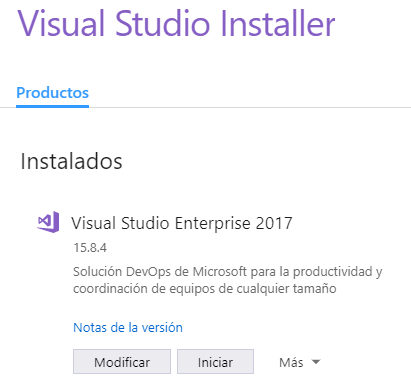
\includegraphics[scale=0.65]{./Figures/PT0.png}
	\caption{Main window of the Visual Studio Installer with the release Enterprise 2017 shown.}
	\label{fig:vsi:list}
\end{figure}

\begin{figure}
	\centering
	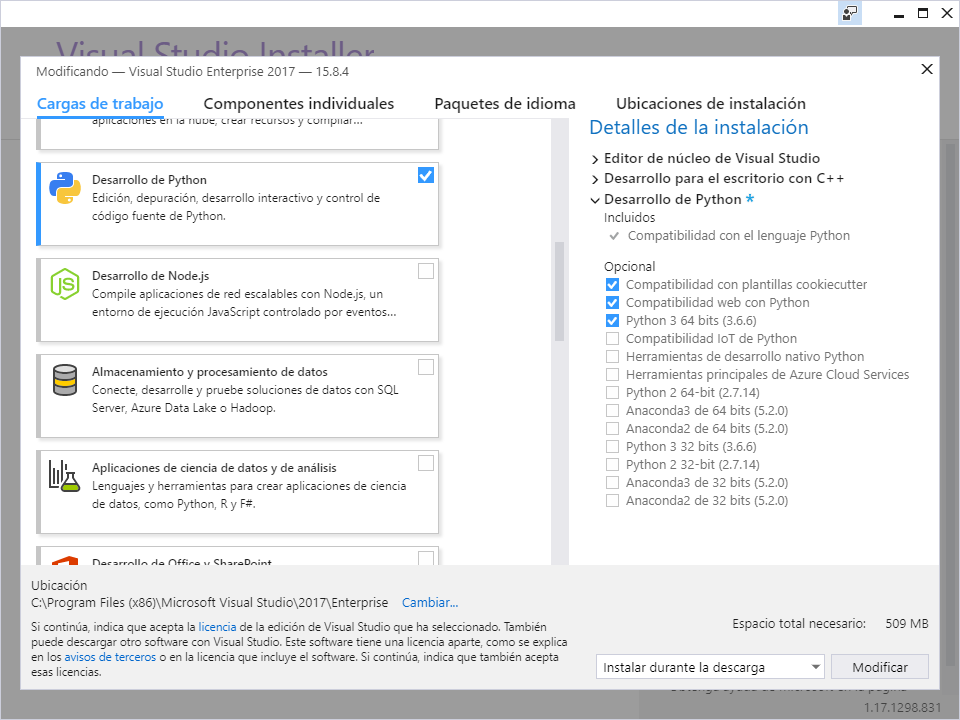
\includegraphics[scale=0.5]{./Figures/PT1V2.png}
	\caption{Workloads ready to be installed using the Visual Studio Installer. The Python development is already selected and the needed characteristics chosen.}
	\label{fig:vsi:mods}
\end{figure}


%This chapter consists of a several steps in order to get embedded Python 
%Project support.
%\begin{enumerate}
%\item Create a new project.
%
%On the top-left corner, check the option 
%\textbf{``FILE{$\rightarrow$}New{$\rightarrow$}Project...''}.
%\item Browse Python templates.
%
%On the newly opened window's left panel, expand the following arrow tree: 
%\textbf{``Installed{$\rightarrow$}Templates{$\rightarrow$}Python''}.
%
%
%
%\item Download additional Python Software.
%
%Hit on \textbf{``Get Python Tools for Visual Studio''} and click on \textbf{OK}.
%\ref{fig:PyStep1}
%%1
%
%
%A new tab will pop-up. Click on \textbf{``Download Python Tools for Visual 
%Studio''}.
%\ref{fig:PyStep2}
%%2
%
%\item Install additional Python Software.
%
%Upon finishing the download an installation will request Administrator 
%permissions, grant them by clicking on \textbf{``Execute''}.
%\ref{fig:PyStep34}
%%34
%
%During the installation wizard the user must accept the License Agreement terms 
%as well as close all Visual Studio running windows.
%
%To finish the installation, click on \textbf{``Finish''}. Run Visual Studio 
%again.
%\ref{fig:PyStep567}
%%567
%
%\item Create a new Python project.
%
%On the top-left corner, go to 
%\textbf{``FILE{$\rightarrow$}New{$\rightarrow$}Project...''} and start a any 
%Python project template on 
%\textbf{Installed{$\rightarrow$}Templates{$\rightarrow$}Python}.
%
%\ref{fig:PyStep8}
%%8
%
%\end{enumerate}
%
%
%\begin{figure}[h]
%    \centering
%    \caption{Selecting new Python Project without Python Tools.}
%    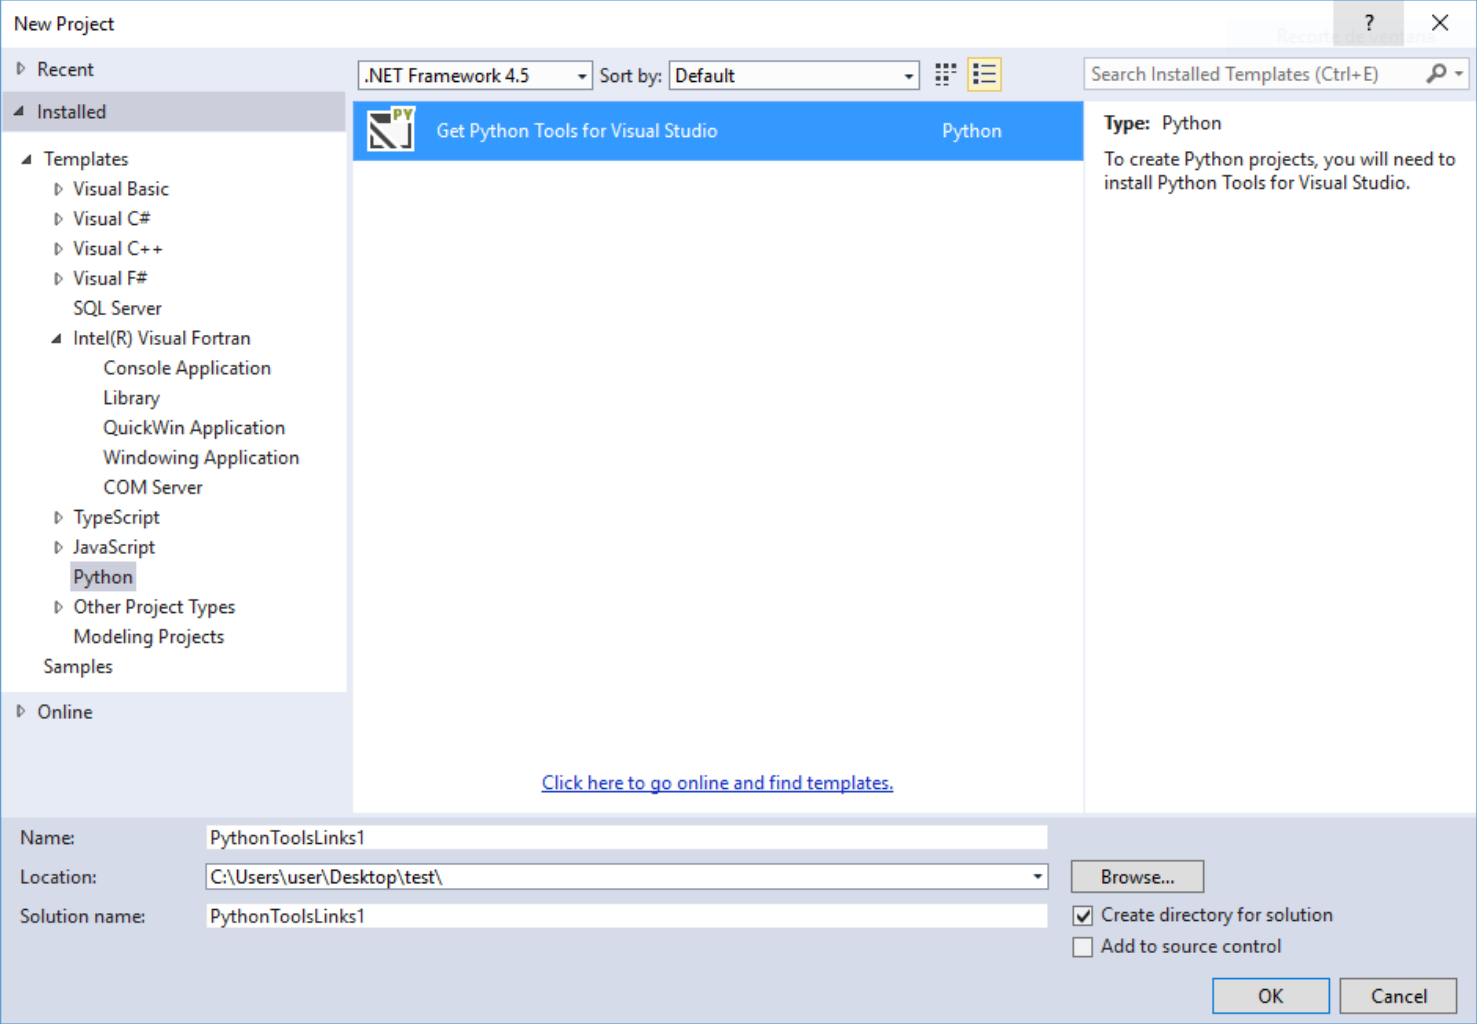
\includegraphics[width= 0.85 \textwidth]{Figures/step1v2.png}
%    \label{fig:PyStep1}
%\end{figure}
%
%
%\begin{figure}[h]
%    \centering
%    \caption{Visual Studio link to Python Tools Installer.}
%    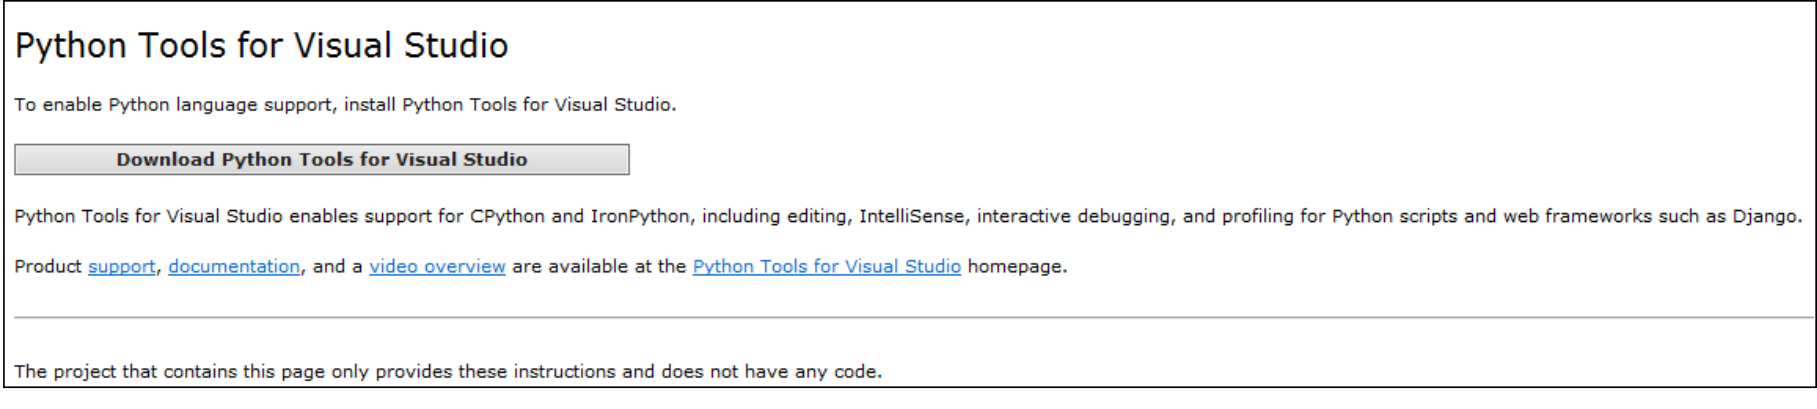
\includegraphics[width= 0.85 \textwidth]{Figures/step2v2.png}
%    \label{fig:PyStep2}
%\end{figure}
%
%\begin{figure}[h]
%\centering
%\caption{Python Tools Programs to be installed.}
%\begin{subfigure}[t]{.5\linewidth}
%\centering
%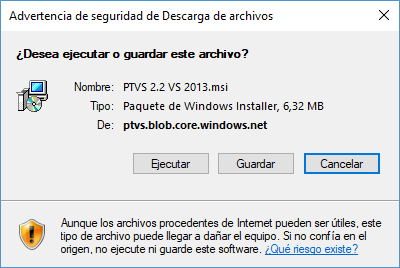
\includegraphics[width= 0.85 \textwidth]{Figures/step3.png}
%\end{subfigure}%
%\begin{subfigure}[t]{.5\linewidth}
%\centering
%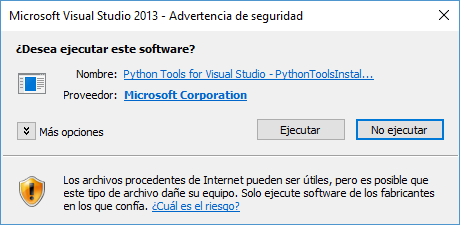
\includegraphics[width= 0.85 \textwidth]{Figures/step4.png}
%\end{subfigure}\\[1ex]
%\label{fig:PyStep34}
%\end{figure}
%
%\begin{figure}[h]
%\caption{Input and warnings from the Installation Setups.}
%\begin{subfigure}{.5\linewidth}
%\centering
%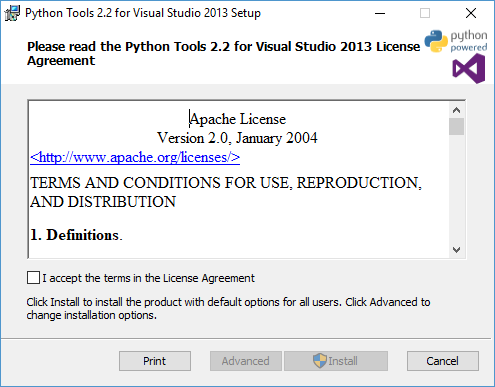
\includegraphics[width= 0.85 \textwidth]{Figures/step5.png}
%\end{subfigure}%
%\begin{subfigure}{.5\linewidth}
%\centering
%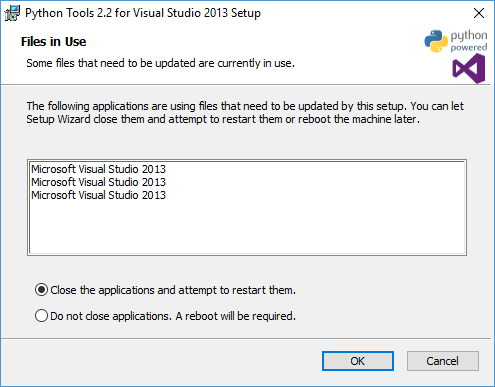
\includegraphics[width= 0.85 \textwidth]{Figures/step6.png}
%\end{subfigure}\\[4ex]
%\begin{subfigure}{\linewidth}
%\centering
%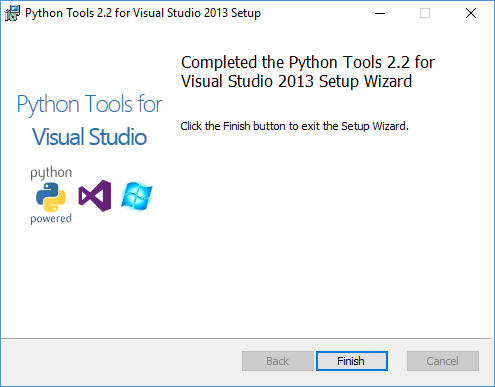
\includegraphics[width= 0.85 \textwidth]{Figures/step7.png}
%\end{subfigure}
%\label{fig:PyStep567}
%\end{figure}
%
%\begin{figure}
%\centering
%\caption{Selecting new Python Project with Python Tools.}
%\begin{normalsize}
%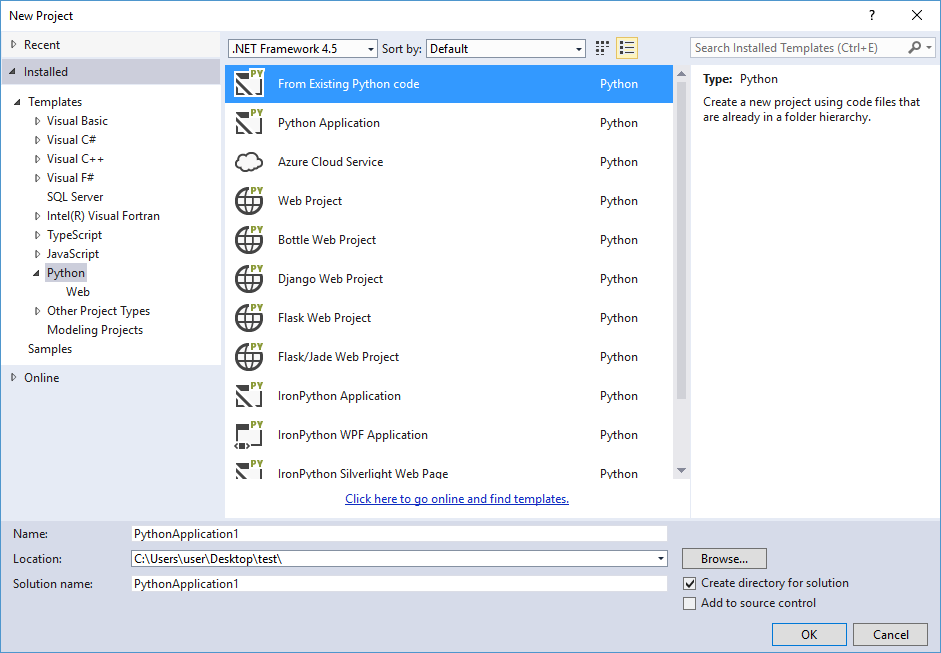
\includegraphics[width= 0.85 \textwidth]{Figures/step8.png}
%\end{normalsize}
%\label{fig:PyStep8}
%\end{figure}
%\clearpage


    
    \section{Create a Python project}

We will see during this guide that the process for creating a new project is similar for all the programming languages, in the case of a Python project:

\begin{enumerate}
	\item Open your version of Visual Studio.
	\item Click on \textit{File/New/Project...}
	\item In the \textit{Python} menu select \textit{Python Application}.
	\item Choose a name for the project (Figure \ref{fig:PP0}).
    \item Change the \textit{Location} of the solution, a directory will be created there.
	\item Select option \textit{Create directory for solution}.
	\item Choose the name of the solution, it does not have to be the same as the name of the project.	
	\item Click on \textit{OK}.
\end{enumerate}

\begin{figure}[h]
    \centering
    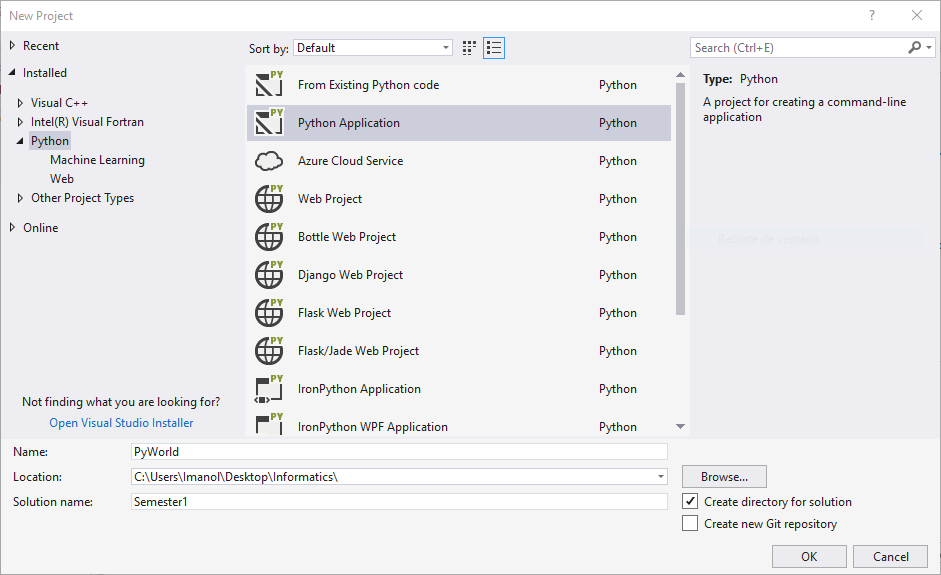
\includegraphics[width= \textwidth]{Figures/PP0V2.png}
    \caption{Window \textit{New Project} where creating a Python project.}
    \label{fig:PP0}
\end{figure}



    \section{Execute the ``Hello World'' example}

This first example ensures that the installation has finished correctly. Like in the rest of the programming languages, it writes a ``Hello World'' message on the console. In this case, there is not a template already written with this example so we will write it from scratch. Open the project created in the previous section, you will find a \texttt{.py} file with the same name as the project, open it and write the following code: %\vskip \baselineskip

\vspace{0.5cm} 
\begin{lstlisting}
     print("Hello World!")
\end{lstlisting}

Now, in order to execute this Python script, the interpreter has to be called for translating it to machine code dynamically:

\begin{enumerate}
	\item Click on \textit{DEBUG/Start Without Debugging} or click on the corresponding icon. The program is then executed on a new command prompt.
\end{enumerate}

\begin{IN}
    More project/solution examples with Python language can be downloaded from:
    
     \url{https://github.com/jahrWork/Visual-Studio-projects}.
\end{IN}

    \section{Installing and removing Python Packages}

Python can download projects developed by other people and include them in our own solutions. These projects or \textbf{packages} have been tested by experts to ensure a proper performance and can help us while coding with no need of developing the code from scratch. In order to install a package follow the next steps:

\newpage
\begin{enumerate}[nosep]
	\item Open your Python Project.
	\item If the Solution Explorer is not opened, click on \textit{View/Solution Explorer}.
	\item Unfold the \textit{Python Environments} menu inside the directory of the specific project in the solution explorer.
	\item Right click on \texttt{Python x.x (xx-bit)} and select \textit{Install Python package...} (Figure \ref{fig:pkg0}).
	\item Type the \textit{Package name} to be installed and press on \textit{Enter} (Figure \ref{fig:pkg1}).
	\item A new window will ask you for \textbf{Administrator privileges} as shown on Figure \ref{fig:pkg15}. Select the third option: \textit{Always elevate when installing or removing packages} and Visual Studio will grant permissions automatically.
    \item The process of downloading and installing starts.
	%\item On the \textit{Solution Explorer} tab on \textit{Solution 
	%%%name/Python Environments/Python x.x (xx-bit)} menu and check if the 
	%%%%\textbf{package} appears ().
\end{enumerate}

\begin{figure}[h]
    \centering
    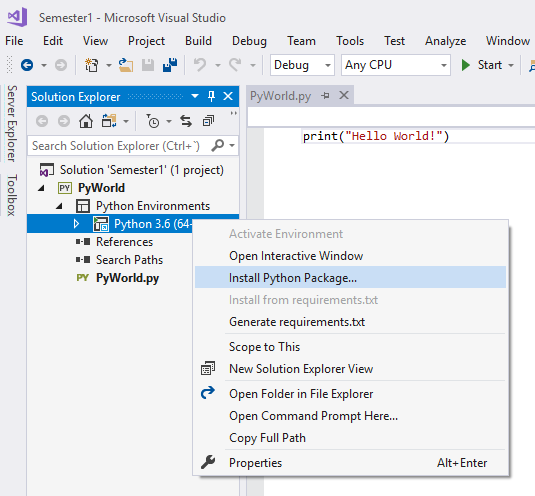
\includegraphics[width= 0.9 \textwidth]{Figures/PPM0V1.png}
    \caption{First step to install new Python packages on the Python environment.}
    \label{fig:pkg0}
\end{figure}

\begin{figure}[h]
    \centering
    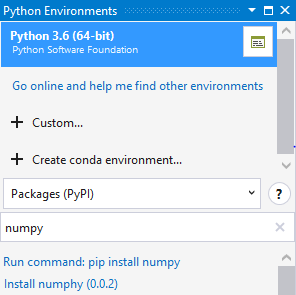
\includegraphics[width=0.6 \textwidth]{Figures/PPM1V2.png}
    \caption{Second step to install new Python packages on the python environment. Write here the name of the package to be installed.}
    \label{fig:pkg1}
\end{figure}

\begin{figure}[h]
	\centering
	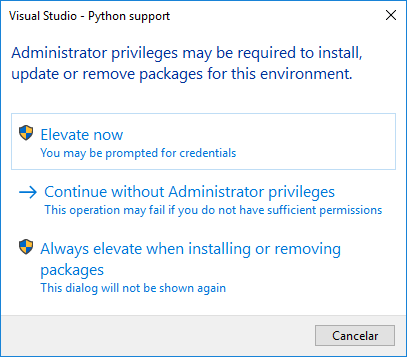
\includegraphics[width=0.6 \textwidth]{Figures/PPM15.png}
	\caption{Confirmation of the administrator privileges in order to install or remove packages. Click on \textit{Always elevate when installing or removing packages}.}
	\label{fig:pkg15}
\end{figure}

\newpage
If a package is not needed anymore, it can be removed from the environment by following the next steps:

\begin{enumerate}
	\item Open a Python Project.
	\item Unfold the \textit{Python Environments/Python x.x (xx-bit)} menu in the Solution Explorer.
	\item Right click on the \textit{Package name} to be removed and select \textit{Remove} (Figure \ref{fig:pkg2}). 
\end{enumerate}

\begin{figure}[h]
    \centering
    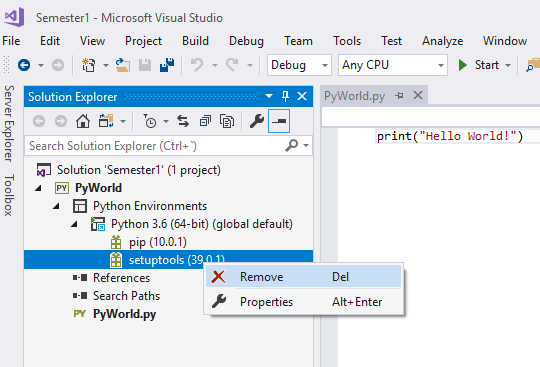
\includegraphics[width= 0.9 \textwidth]{Figures/PPM2V1.png}
    \caption{Option reserved for removing those Python packages not needed from the Python environment.}
    \label{fig:pkg2}
\end{figure}

%\section{Configuring a Python Environment}
%
%In previous sections we've seen how to create Python projects with the default configuration of VS. As opposed to Fortran projects where a unique compiler makes use of selected source files, Python projects execute an script and the required source files with a configurable \textbf{Python Environment}. This environment is composed by the \textbf{Python Interpreter}, which specifies the programming language version (2.7, 3.5, 3.6, etc.), and the \textbf{installed packages} from other sources.
%
%On the \textbf{``Solution Explorer''} panel, check whether the \textbf{``Python 
%Environment''} option is expandable and contains a suitable environment.
%
%If affirmative, no more further steps are required, else continue to the 
%following step.
%
%\begin{enumerate}
%
%\item Right-click on \textbf{``Python Environment''} and select 
%\textbf{``Add/Remove Python Environments''}.
%\ref{fig:PyStep9}
%%9
%
%\begin{figure}[h]
%\centering
%\caption{Add a new Environment.}
%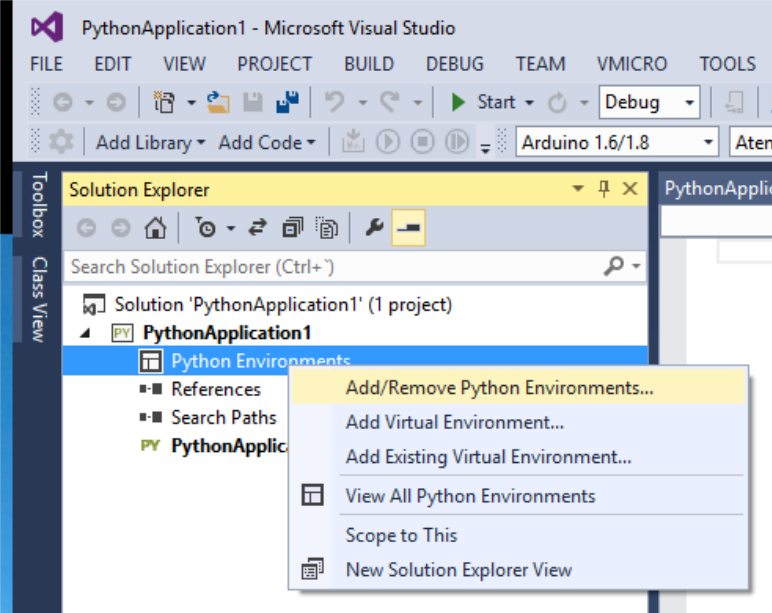
\includegraphics[width=0.85 \textwidth]{Figures/step9v2.png}
%\label{fig:PyStep9}
%\end{figure}
%
%\item Select an environment of your choice if any, and click on \textbf{``OK''}.
%\ref{fig:PyStep10}
%%10
%
%\begin{figure}[h]
%\centering
%\caption{Available Python Environments}
%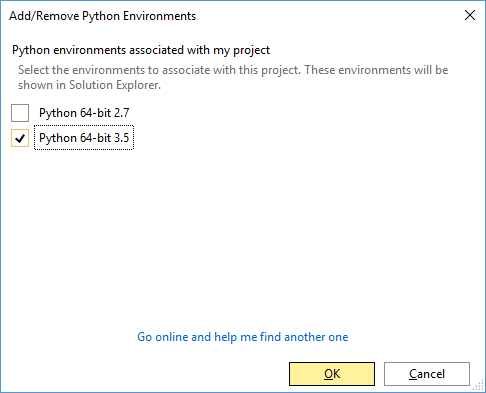
\includegraphics[width=0.85 \textwidth]{Figures/step10.png}
%\label{fig:PyStep10}
%\end{figure}
%
%\end{enumerate}
%
%\section{Configure a custom Python Environment}
%
%It may happen that no environment has been detected or that the selected one 
%does not work (a warning icon is displayed next to it). In these cases a custom 
%configuration is needed.
%
%\begin{enumerate}
%
%\item Open the \textbf{``Python Environments''} panel by clicking on 
%\textbf{``VIEW{$\rightarrow$}Other Windows{$\rightarrow$}Python Environments''}.
%
%\item Select \textbf{``Custom...''}. Configure all the fields with your custom 
%installation. Click on \textbf{Apply} to save the changes. 
%\ref{fig:PyStep11}
%%11
%
%\begin{figure}[h]
%\centering
%\caption{Custom Python Environment installed on shared partition.}
%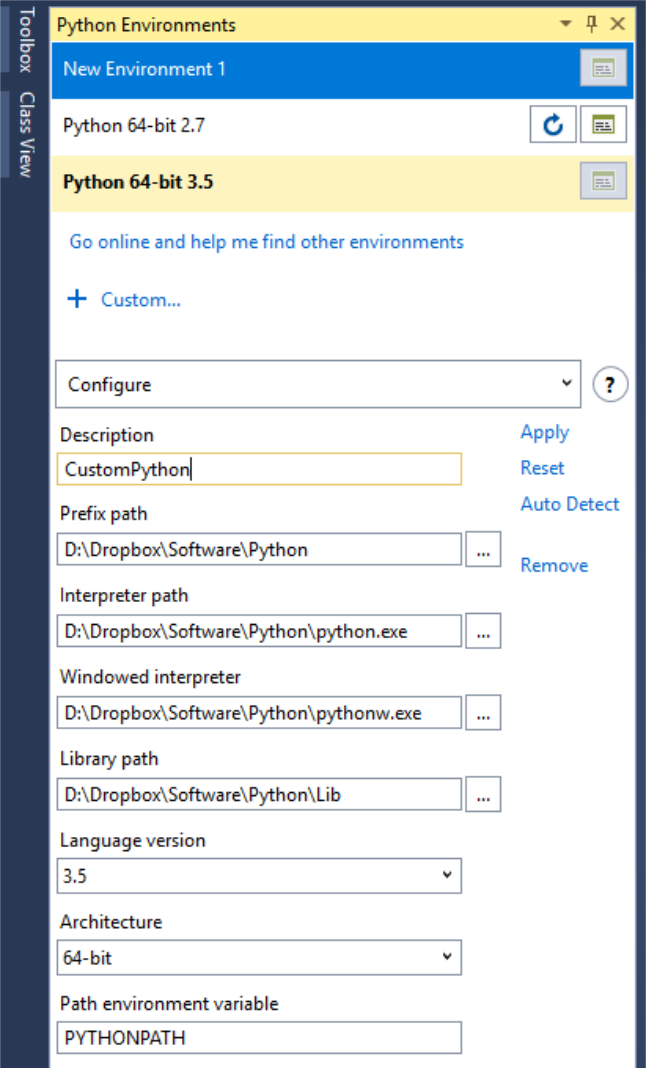
\includegraphics[width=0.75 \textwidth]{Figures/step11v2.png}
%\label{fig:PyStep11}
%\end{figure}
%
%\item On the \textbf{``Solution Explorer''} panel,right-click on 
%\textbf{``Python Environment''} and select \textbf{``Add/Remove Python 
%Environments''}. Select the newly created environment and hit the \textbf{OK} 
%button.
%\ref{fig:PyStep12}
%%12
%
%\begin{figure}[h]
%\centering
%\caption{New custom Python Environments available.}
%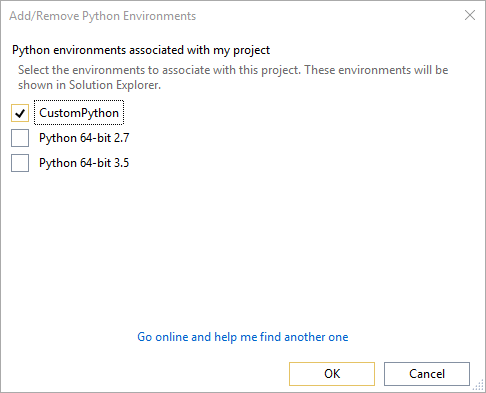
\includegraphics[width=0.85 \textwidth]{Figures/step12.png}
%\label{fig:PyStep12}
%\end{figure}
%
%\end{enumerate}
%
%%---------


%Sometimes due to Visual Studio not finding a suitable Python installation it is 
%necessary to edit the default configuration.
%
%The malfunctioning tents to happen with custom Python installations on 
%non-regular directories or Visual Studio selecting partially removed previous 
%working folders.
%
%If your project does not run properly when hitting the \textbf{``Start''} 
%button you must consider following this chapter's instructions.

%\section{Select a Python Environment}
%
%A Python Environment consists of the following elements.
%\begin{itemize}
%\item A python compiler \textbf{python(.exe)}, version 2.X or 3.X. Executes 
%python scripts.
%\item A python windowed interpreter \textbf{pythonw(.exe)}, which executes 
%commands written on a terminal.
%\item A python \textbf{library folder} where modules and package manager such 
%as \textit{pip} or \textit{easy\_install} are located.
%\end{itemize}
%
%All the elements must be located and correctly bound to the Operating System's 
%programs and libraries. This means that copy-pasting a certain module folder to 
%another environment will not work.
%
%On the \textbf{``Solution Explorer''} panel, check whether the \textbf{``Python 
%Environment''} option is expandable and contains a suitable environment.
%
%If affirmative, no more further steps are required, else continue to the 
%following step.
%
%\begin{enumerate}
%
%\item Right-click on \textbf{``Python Environment''} and select 
%\textbf{``Add/Remove Python Environments''}.
%\ref{fig:PyStep9}
%%9
%
%\begin{figure}[h]
%\centering
%\caption{Add a new Environment.}
%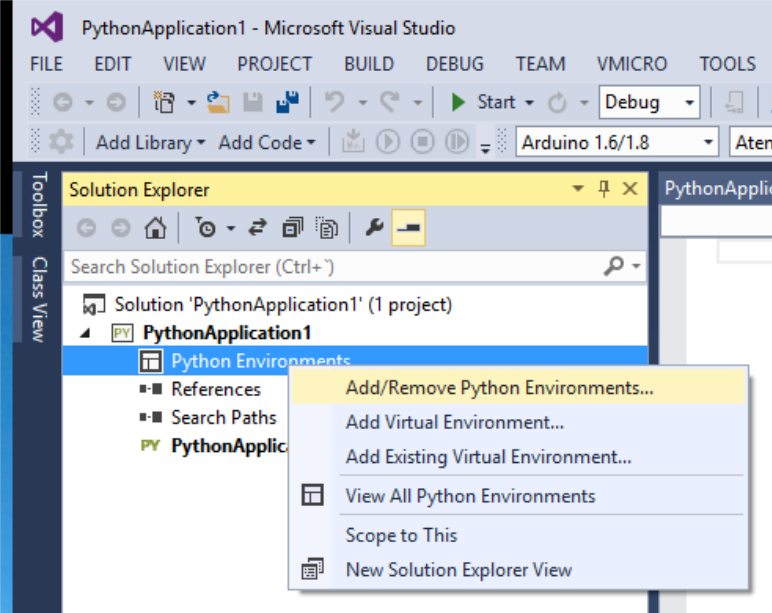
\includegraphics[width=0.85 \textwidth]{Figures/step9v2.png}
%\label{fig:PyStep9}
%\end{figure}
%
%\item Select an environment of your choice if any, and click on \textbf{``OK''}.
%\ref{fig:PyStep10}
%%10
%
%\begin{figure}[h]
%\centering
%\caption{Available Python Environments}
%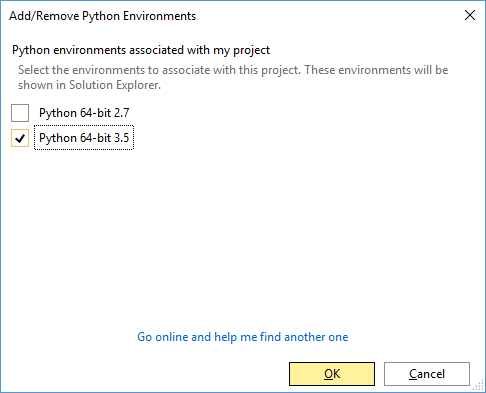
\includegraphics[width=0.85 \textwidth]{Figures/step10.png}
%\label{fig:PyStep10}
%\end{figure}
%
%\end{enumerate}
%
%\section{Configure a custom Python Environment}
%
%It may happen that no environment has been detected or that the selected one 
%does not work (a warning icon is displayed next to it). In these cases a custom 
%configuration is needed.
%
%\begin{enumerate}
%
%\item Open the \textbf{``Python Environments''} panel by clicking on 
%\textbf{``VIEW{$\rightarrow$}Other Windows{$\rightarrow$}Python Environments''}.
%
%\item Select \textbf{``Custom...''}. Configure all the fields with your custom 
%installation. Click on \textbf{Apply} to save the changes. 
%\ref{fig:PyStep11}
%%11
%
%\begin{figure}[h]
%\centering
%\caption{Custom Python Environment installed on shared partition.}
%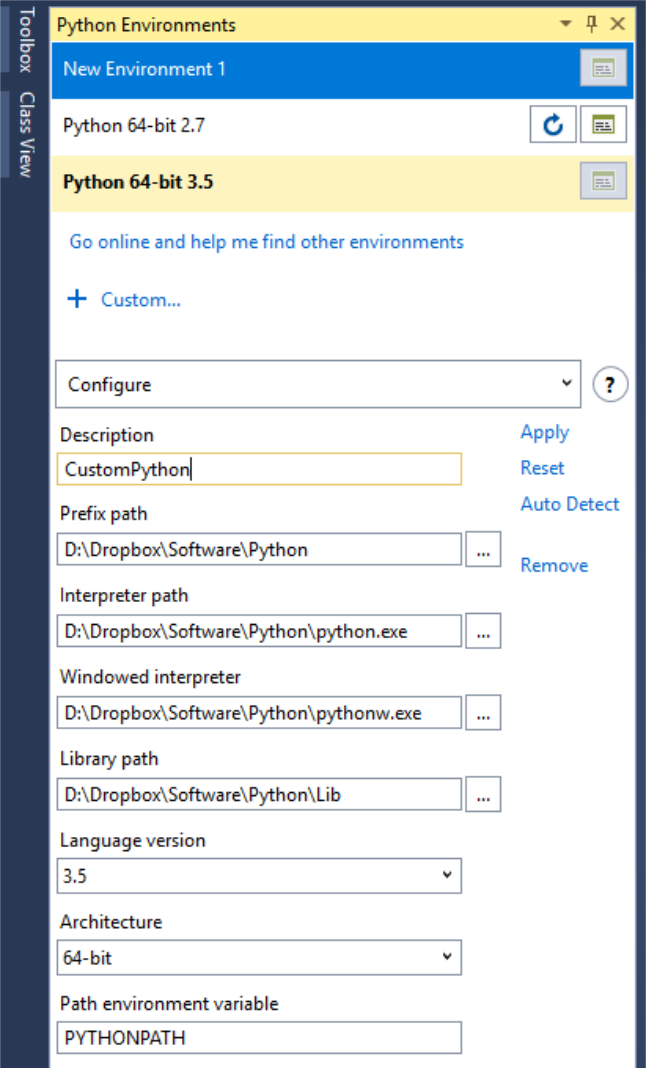
\includegraphics[width=0.75 \textwidth]{Figures/step11v2.png}
%\label{fig:PyStep11}
%\end{figure}
%
%\item On the \textbf{``Solution Explorer''} panel,right-click on 
%\textbf{``Python Environment''} and select \textbf{``Add/Remove Python 
%Environments''}. Select the newly created environment and hit the \textbf{OK} 
%button.
%\ref{fig:PyStep12}
%%12
%
%\begin{figure}[h]
%\centering
%\caption{New custom Python Environments available.}
%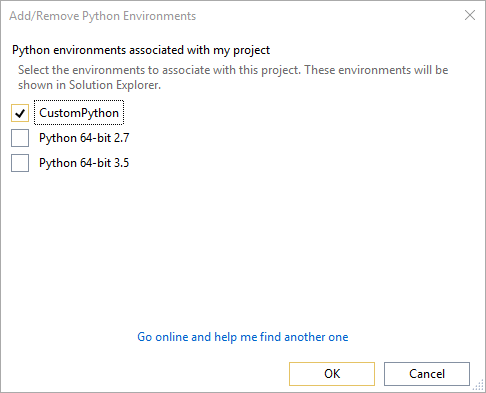
\includegraphics[width=0.85 \textwidth]{Figures/step12.png}
%\label{fig:PyStep12}
%\end{figure}
%
%\end{enumerate}

    \section{Include modules \& packages from other Projects}

Python Projects can ``import'' modules and packages from other projects on separated directories. With this way we can have the latest updates of an actively developed module or package without duplicating code. There are two ways for including external modules and packages:

\subsection*{Modules/Packages from the same solution}

\begin{itemize}
	\item In the solution explorer, in a project, right click on \textit{References} and select \textit{Add Reference...}
	\item Check Python Projects in order to import their modules and packages as shown on Figure \ref{fig:refs0}.
\end{itemize}

\begin{figure}[h]
    \centering
    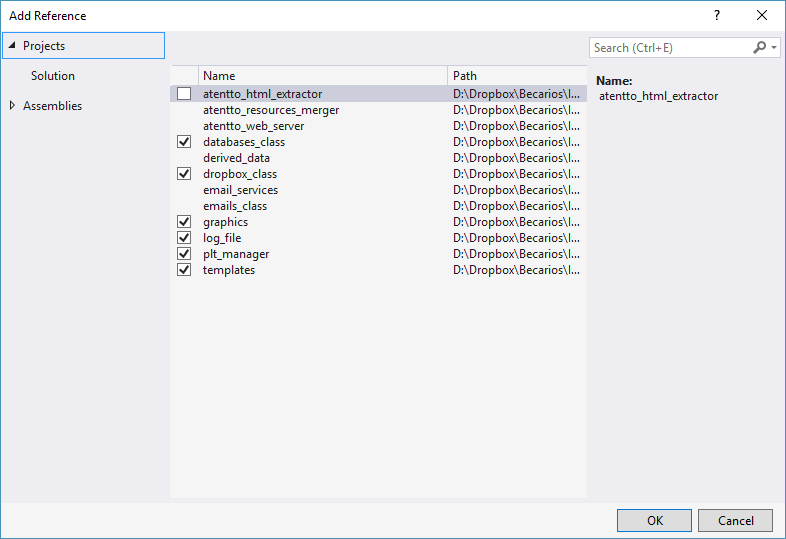
\includegraphics[width= \textwidth]{Figures/PPR0.png}
    \caption{Available Python Projects for importing packages. Each project contains a package with the same name on its root directory.}
    \label{fig:refs0}
\end{figure}

\subsection*{Modules/Packages outside solution}

\begin{itemize}
	\item In the solution explorer, in a project, right click on \textit{Search Paths} and select \textit{Add Folder to Search Path...}
	\item Select the root folder where the Python module/package to be imported is located (see Figure \ref{fig:refs1}).
\end{itemize}

\begin{figure}[h]
    \centering
    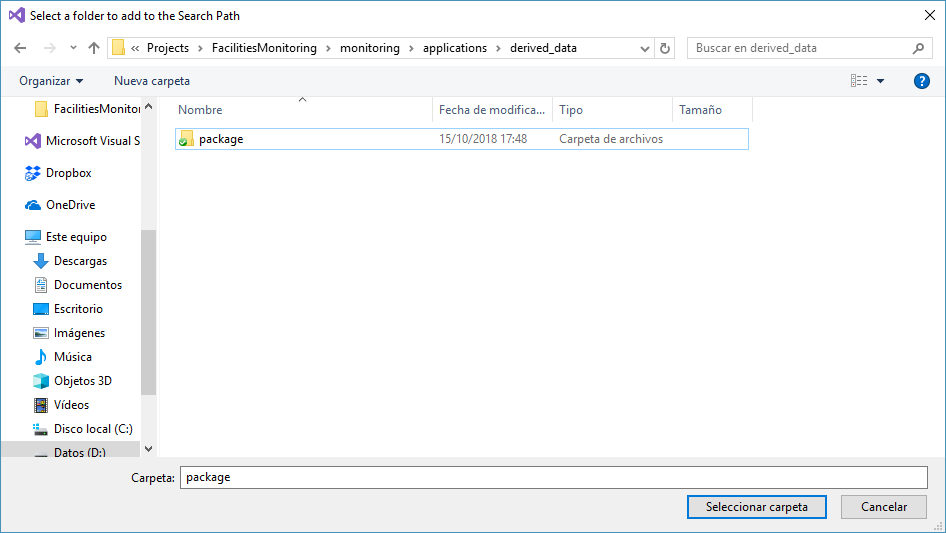
\includegraphics[width=\textwidth]{Figures/PPR1.png}
    \caption{In this window we can look for the path of the package to be used by the Python Project.}
    \label{fig:refs1}
\end{figure}
